%%%%%%%%%%%%%%%%%%%%%%%%%%%%%%%%%%%%%%%%%
% Plasmati Graduate CV
% LaTeX Template
% Version 1.0 (24/3/13)
%
% This template has been downloaded from:
% http://www.LaTeXTemplates.com
%
% Original author:
% Alessandro Plasmati (alessandro.plasmati@gmail.com)
%
% License:
% CC BY-NC-SA 3.0 (http://creativecommons.org/licenses/by-nc-sa/3.0/)
%
% Important note:
% This template needs to be compiled with XeLaTeX.
% The main document font is called Fontin and can be downloaded for free
% from here: http://www.exljbris.com/fontin.html
%
%%%%%%%%%%%%%%%%%%%%%%%%%%%%%%%%%%%%%%%%%

%----------------------------------------------------------------------------------------
%	PACKAGES AND OTHER DOCUMENT CONFIGURATIONS
%----------------------------------------------------------------------------------------

\documentclass[a4paper,10pt]{article} % Default font size and paper size

\usepackage{fontspec} % For loading fonts
\defaultfontfeatures{Mapping=tex-text}
%\setmainfont[SmallCapsFont = Fontin SmallCaps]{Fontin} % Main document font

\usepackage{xunicode,xltxtra,url,parskip} % Formatting packages

\usepackage[usenames,dvipsnames]{xcolor} % Required for specifying custom colors

\usepackage[big]{layaureo} % Margin formatting of the A4 page, an alternative to layaureo can be \usepackage{fullpage}
% To reduce the height of the top margin uncomment: \addtolength{\voffset}{-1.3cm}

\usepackage{hyperref} % Required for adding links	and customizing them
\definecolor{linkcolour}{rgb}{0,0.2,0.6} % Link color
\hypersetup{colorlinks,breaklinks,urlcolor=linkcolour,linkcolor=linkcolour} % Set link colors throughout the document

\usepackage{titlesec} % Used to customize the \section command
\titleformat{\section}{\Large\scshape\raggedright}{}{0em}{}[\titlerule] % Text formatting of sections
\titlespacing{\section}{0pt}{3pt}{3pt} % Spacing around sections

\begin{document}

\pagestyle{empty} % Removes page numbering

\font\fb=''[cmr10]'' % Change the font of the \LaTeX command under the skills section

%----------------------------------------------------------------------------------------
%	NAME AND CONTACT INFORMATION
%----------------------------------------------------------------------------------------

\noindent
\par{\centering{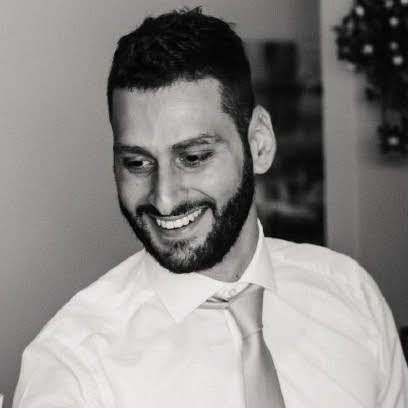
\includegraphics[scale=0.15]{photo.jpg}}\par}
\small

\par{\centering{\Huge Carmelo \textsc{La Gamba}}\bigskip\par} % Your name

\section{Dati personali}

\begin{tabular}{rl}
\textsc{Luogo e data di nascita:} & Vibo Valentia, 20 Aprile 1990 \\
\textsc{Indirizzo:} & via Vincenzo Porri 9, 10153, Torino \\
\textsc{Patente:} & B - Automunito \\
\textsc{Telefono:} & +39 347 64 38 729 \\
\textsc{e-mail:} & \href{mailto:carmelolagamba90@gmail.com}{carmelolagamba90@gmail.com}\\
\textsc{LinkedIn:} & \href{https://www.linkedin.com/in/carmelolagamba/}{www.linkedin.com/in/carmelolagamba/}
\end{tabular}

%----------------------------------------------------------------------------------------
%	WORK EXPERIENCE 
%----------------------------------------------------------------------------------------

\section{Esperienze professionali}

\begin{tabular}{r|p{11cm}}
\textsc{Ott 2019 - Corrente} & Technical Team Leader in \textsc{Altran Italia S.p.A.}, Torino \emph{}\\
& \footnotesize{Progettazione architetture software a microservizi cloud-native. Coordino due team su progetti in ambito finance. Lo sviluppo viene gestito attraverso una metodologia Agile (Scrum).}\\
& \footnotesize{Attività principali: progettazione e sviluppo di microservices in modalità DevOps utilizzando \textbf{Docker, Jenkins, Heroku, OpenShift}, progettazione e sviluppo di cluster \textbf{MongoDB}, gestione architettura front-end in \textbf{Angular8+} }\\
& \footnotesize{Tecnologie e framework usati: \textbf{Docker, Jenkins, Heroku, OpenShift, Java 8, Hibernate, Spring, SpringBoot, Postgres, MongoDB, Angular8+, Git, Gitlab} }\\
\multicolumn{2}{c}{} \\

%------------------------------------------------

\textsc{Ott 2016 - Ott 2019} & Full-stack Software Engineer in \textsc{Sintea Servizi Informatici, gruppo Previnet S.p.a}, Torino \emph{}\\
& \footnotesize{Sviluppo e progettazione di soluzioni software in ambito healthcare attraverso l'utilizzo di un'architettura a microservices. Lo sviluppo viene gestito attraverso una metodologia Agile (Scrum). }\\
& \footnotesize{Attività principali: progettazione e sviluppo di microservices tramite l'utilizzo di \textbf{Spring-Boot e EJB}, progettazione e sviluppo di cluster \textbf{MongoDB}, gestione architettura front-end in \textbf{AngularJS e Angular 2+} }\\
& \footnotesize{Tecnologie e framework usati: \textbf{Java 8, EJB, Hibernate, Spring, SpringBoot, Postgres, MongoDB, Wildfly 10, AngularJS, Angular2+, Git, Jenkins} }\\
\multicolumn{2}{c}{} \\

%------------------------------------------------

\textsc{Giu 2015 - Ott 2016} & Full-stack Software Developer in \textsc{Audacia Srl}, Torino \emph{}\\
& \footnotesize{Sviluppo e progettazione di soluzioni software in ambito assicurativo. Lo sviluppo viene gestito attraverso una metodologia Agile. }\\
& \footnotesize{Attività principali: progettazione e sviluppo di web application utilizzando \textbf{Node.js, Loopback e AngularJS}, sviluppo su db \textbf{NoSQL orientato a grafo ArangoDB}, studio di fattibilità, progettazione e successivo sviluppo di un software per analisi e semantica di testi in ambito assicurativo, scritto in \textbf{Java} utilizzando \textbf{OpenNLP}, una libreria open-source per il \textbf{natural language processing (NLP)}}\\
& \footnotesize{Tecnologie e framework usati: \textbf{Node.js, Loopback, Angular.js, ArangoDB, Java 7, OpenNLP} }\\
\multicolumn{2}{c}{} \\

\end{tabular}

%----------------------------------------------------------------------------------------
%	EDUCATION
%----------------------------------------------------------------------------------------

\section{Titoli di studio}

\begin{tabular}{rl}	
\textsc{Gen 2013 - Mag 2015} & Laurea magistrale in \textsc{Informatica}, \textbf{Università della Calabria}, Rende(CS)\\
& 104/110\\
& Tesi: ``Parallelizzazione CUDA della libreria per automi cellulari OpenCAL''\\
&\textbf{ Esperienze all'estero}: Erasmus+ presso l'Università AGH di Krakow.\\
& Collaborazione con il dipartimento di Computer Science per la tesi sperimentale\\
&\\

%------------------------------------------------

\textsc{Ott 2009 - Dic 2012} & Laurea triennale in \textsc{}\textsc{Informatica}, \normalsize\textbf{Università della Calabria}, Rende (CS)\\
 &101/110\\
& Tesi: ``Realizzazione di un sistema di inter-scambio tra strumenti \\
&per il Project
Management" \\
&\\
\end{tabular}

%----------------------------------------------------------------------------------------
%	SCHOLARSHIPS AND ADDITIONAL INFO
%----------------------------------------------------------------------------------------

\section{Corsi e certificazioni}

\begin{tabular}{rl}
\textsc{Mag} 2018 & \textsc{Machine Learning},  Coursera: \textbf{ID 9PBTUP3QG2AG}\\
\textsc{Apr} 2019 & \textsc{Functional Programming Principles in Scala},  Coursera: \textbf{ID LS7WXPYGKSZX}\\
\textsc{Mag} 2019 & \textsc{Functional Program Design in Scala},  Coursera: \textbf{ID GTUWGVELYJPR}
\end{tabular}

%----------------------------------------------------------------------------------------
%	LANGUAGES
%----------------------------------------------------------------------------------------

\section{Lingua}

\begin{tabular}{rl}
\textsc{Italian:} & Madrelingua\\
\textsc{English:} & Buono, affinato con esperienza all'estero
\end{tabular}

%----------------------------------------------------------------------------------------
%	Soft SKILLS 
%----------------------------------------------------------------------------------------

\section{Soft Skills}

\begin{tabular}{lr}
Capacità di lavorare in team, proattività, capacità nelle relazioni, problem solving, \\
adattabilità, capacità di lavorare per obiettivi
\end{tabular}

%----------------------------------------------------------------------------------------
%	INTERESTS AND ACTIVITIES
%----------------------------------------------------------------------------------------

\section{Interessi e attività}

Nuove tecnologie, Machine Learning, Modelli matematici applicati, Parallel computing\\
IoT, Artificial Intelligence, Automotive, Industria 4.0, Domotica\\
Studio di strumenti musicali (chitarra classica, acustica)\\
Sport (nuoto e pallavolo)

%----------------------------------------------------------------------------------------

\section{}
Autorizzo il trattamento dei dati personali contenuti nel mio curriculum vitae in base all’art. 13 del D. Lgs. 196/2003 e all’art. 13 del Regolamento UE 2016/679 relativo alla protezione delle persone fisiche con riguardo al trattamento dei dati personali.

\end{document}
